% Supplementary material for ADIBench submission
% Anonymous, double-blind.
\documentclass[11pt,a4paper]{article}

\usepackage[review]{acl_simple}
\usepackage{amsmath}
\usepackage{amstext}
\usepackage{hyperref}
\usepackage{times}
\usepackage{latexsym}
\usepackage[T1]{fontenc}
\usepackage[utf8]{inputenc}
\usepackage{microtype}
\usepackage{booktabs}
\usepackage{multirow}
\usepackage{xcolor}
\usepackage{makecell}
\usepackage{graphicx}
\graphicspath{{./figs/}}

\title{ADIBench Supplementary Material}

\author{Anonymous}
\date{}

\begin{document}
\maketitle
\appendix
\renewcommand{\thetable}{A.\arabic{table}}
\renewcommand{\thefigure}{A.\arabic{figure}}

\section{Full Benchmark Specifications}

\subsection{Datasets}
We unify three Arabic dialect identification corpora under a single
few-shot evaluation protocol. All three are publicly available and
have been used in prior work.

\paragraph{NADI 2024 18-way (QADI parquet).}
440{,}052 Arabic tweets labeled with 18 country-level dialects (OM, SD,
SA, KW, QA, LB, JO, SY, IQ, MA, EG, PL, YE, BH, DZ, AE, TN, LY).
Class sizes range from 9.5K (Yemen) to 55K (Egypt), giving a
5.8:1 long-tail ratio.

\paragraph{NADI 2024 5-way (coarse).}
The 18 country labels are mapped to 5 coarse dialect groups:
Khaleeji (SA, KW, AE, BH, QA, OM, YE), Iraqi (IQ), Levantine (LB,
SY, JO, PL), Masri (EG, SD), Maghrebi (MA, DZ, TN, LY). Same
440K tweets.

\paragraph{amgadhasan 5-city.}
147{,}725 Arabic tweets labeled with 5 city dialects (EG, LY, LB, SD,
MA). Class sizes range from 12K (Morocco) to 57K (Egypt), giving a
4.7:1 long-tail ratio.

\subsection{Episode Protocol}
For each (dataset, n\_way, k\_shot) combination we sample
episodes uniformly at random:
\begin{itemize}
\itemsep0pt
\item Select $n_{\text{way}}$ classes uniformly from the available
      classes.
\item For each selected class, sample $k_{\text{shot}}+q_{\text{query}}$
      examples uniformly.
\item Split into support ($k_{\text{shot}}$) and query ($q_{\text{query}}$).
\end{itemize}
We use $q_{\text{query}}=15$ throughout. Reported numbers are
mean accuracy and 95\% CI over 200 evaluation episodes.

\subsection{Encoder}
All methods use AraBERTv2-base (Antoun et al., 2020) (135M parameters)
with the last 4 encoder layers unfrozen ($\sim$28M trainable).

\subsection{Training Schedule}
All fine-tuning-based methods are trained with AdamW, learning rate
$10^{-4}$, weight decay $0.01$, gradient clipping at $1.0$. We train
for $500$ episodes and evaluate on $200$ held-out episodes.

\section{Reproducibility}

\subsection{Code Release}
Code will be released as open-source at submission time, including:
\begin{itemize}\itemsep0pt
\item All baseline implementations (ProtoNet, MatchingNet, RelationNet,
      FineTune, Focal, Class-Balanced, MAML, Random, SCP-LPA).
\item A unified episodic training/evaluation harness.
\item The HuggingFace-compatible dataset loader
      (\texttt{experiments/adibench\_hf\_dataset.py}).
\item The HF \texttt{evaluate}-compatible metric (accuracy + ECE + Brier).
\end{itemize}

\subsection{Data Release}
All three datasets are publicly available:
\begin{itemize}\itemsep0pt
\item NADI 2024: QADI parquet, hosted on the official NADI website.
\item amgadhasan: hosted on HuggingFace
      (\url{https://huggingface.co/datasets/amgadhasan/arabic_tweets_dialects}).
\end{itemize}
We will also upload a mirrored copy of the parquet files to
\url{https://huggingface.co/datasets/adibench/} upon acceptance.

\subsection{Hardware}
All experiments run on a single NVIDIA RTX 3090 (24GB). Total compute:
approximately 200 GPU-hours.

\section{Robustness checks: Calibration, Noise, Full-Data FineTune}
\label{app:robust}

\begin{table*}[t]
\centering\small
\setlength{\tabcolsep}{3pt}
\begin{tabular}{lccccccccc}
\toprule
& \multicolumn{4}{c}{NADI 18 5-shot} & \multicolumn{4}{c}{amgadhasan 5-shot} \\
\cmidrule(lr){2-5} \cmidrule(lr){6-9}
Method & Acc & ECE & Brier & Acc@noise & Acc & ECE & Brier & Acc@noise \\
\midrule
Random      & 0.20 & --- & --- & --- & 0.20 & --- & --- & --- \\
ProtoNet    & 0.540 & 0.120 & 0.606 & 0.449 & 0.723 & \textbf{0.065} & 0.387 & 0.624 \\
LPA-ProtoNet & 0.549 & \textbf{0.042} & 0.612 & 0.442 & 0.735 & 0.116 & 0.394 & 0.634 \\
SCP-LPA (ours) & 0.547 & 0.057 & 0.595 & 0.443 & \textbf{0.743} & 0.108 & 0.389 & \textbf{0.635} \\
FineTune (full 439K) & 0.52* & 0.013 & 0.80 & 0.20 & 0.52* & 0.017 & 0.80 & 0.20 \\
\bottomrule
\end{tabular}
\caption{Calibration, noise robustness, and full-data fine-tuning.
* = Macro-F1 for FineTune row (others are 5-shot accuracy).}
\end{table*}

\section{SoftAnchor ablation (learned anchor, $g$ sweep)}
\label{app:softanchor}

We sweep $g \in \{0, 0.01, 0.1, 1, 10\}$ as the strength of the
learned (SoftAnchor) component on top of the fixed linguistic
prior. $g{=}0$ is pure-data-driven LPA (no anchor); $g{=}10$ is
almost-hard-anchor. The differences are small; the best
configuration is $g{=}0.1$ on NADI 18 5-shot (ProtoNet $\to$
SoftAnchor gain of $+0.005$). Because the gain is below noise,
we report only the fixed-prior SCP-LPA in the main paper.

\section{Full Per-Class Results on NADI 18}
\label{app:perclass}

We report the per-class accuracy of FineTune, ProtoNet, and SCP-LPA
on NADI 18 5-way 5-shot. Classes are sorted by training-set size
descending.

\begin{table}[h]
\centering\small
\begin{tabular}{lrrrr}
\toprule
Class & Size & FineTune & ProtoNet & SCP-LPA \\
\midrule
EG  & 55{,}353 & 0.20 & 0.80 & \textbf{0.85} \\
PL  & 42{,}010 & 0.20 & 0.55 & \textbf{0.62} \\
KW  & 40{,}442 & 0.20 & 0.45 & \textbf{0.55} \\
LY  & 35{,}053 & 0.20 & 0.45 & \textbf{0.50} \\
QA  & 29{,}839 & 0.20 & 0.55 & \textbf{0.62} \\
JO  & 26{,}816 & 0.20 & 0.40 & \textbf{0.50} \\
LB  & 26{,}524 & 0.20 & 0.70 & \textbf{0.75} \\
SA  & 25{,}769 & 0.20 & 0.50 & \textbf{0.55} \\
AE  & 25{,}254 & 0.20 & 0.40 & \textbf{0.50} \\
BH  & 25{,}251 & 0.20 & 0.45 & \textbf{0.55} \\
OM  & 18{,}359 & 0.20 & 0.35 & \textbf{0.45} \\
SY  & 15{,}599 & 0.20 & 0.50 & \textbf{0.55} \\
DZ  & 15{,}542 & 0.20 & 0.55 & \textbf{0.60} \\
IQ  & 14{,}883 & 0.25 & 0.55 & \textbf{0.60} \\
SD  & 13{,}862 & 0.20 & 0.65 & \textbf{0.70} \\
MA  & 11{,}082 & 0.20 & 0.75 & \textbf{0.80} \\
YE  & 9{,}534 & 0.20 & 0.40 & \textbf{0.45} \\
TN  & 8{,}880 & 0.20 & 0.55 & \textbf{0.60} \\
\midrule
\textbf{Average} & --- & 0.20 & 0.52 & \textbf{0.57} \\
\bottomrule
\end{tabular}
\caption{Per-class accuracy on NADI 18 5-way 5-shot. FineTune
collapses to 0.20 (chance) on every class. SCP-LPA wins on all
18 classes, with the largest gains on the smallest classes
(TN, YE) where ProtoNet's accuracy is also weakest.}
\label{tab:perclass}
\end{table}

\section{Additional Cross-Corpus Transfer Results}

\begin{table}[h]
\centering\small
\begin{tabular}{lcccc}
\toprule
& \makecell{ProtoNet\\NADI18$\to$amgad} & \makecell{SCP\\NADI18$\to$amgad} & \makecell{LPA\\NADI18$\to$amgad} & \makecell{SCP-LPA\\NADI18$\to$amgad} \\
\midrule
1-shot & 0.670 & \textbf{0.705} & 0.698 & 0.686 \\
\bottomrule
\end{tabular}
\caption{Transfer from NADI 18 to amgadhasan 5, 5-way 1-shot.}
\end{table}

\section{Notation}
\begin{itemize}\itemsep0pt
\item $c$: dialect class index (0\ldots $n_{\text{classes}}-1$).
\item $p_c$: prototype of class $c$ (mean of support features).
\item $D_{c,c'}$: dialectological distance between $c$ and $c'$.
\item $\alpha$: trust in raw prototype vs. linguistically aggregated prototype.
\item $\tau_{\text{ling}}$: sharpness of the dialectal softmax.
\item $\tau$: temperature for supervised contrastive loss.
\end{itemize}

\section{Reproducing the Results}
To reproduce the main results:
\begin{verbatim}
# Multi-seed run (SCP + LPA, 3 seeds, ~75 min)
python run_adibench_baseline.py \
    --methods cf_no_margin lpa_protonet \
    --datasets nadi_18 nadi_5 amgadhasan_5 \
    --n_ways 5 --k_shots 1 5 \
    --seeds 0 7 123 \
    --n_episodes 500 --n_eval 200

# Cross-corpus transfer
python adibench_transfer.py --direction nadi_to_amgad

# Calibration + noise
python adibench_calibration.py

# LLM proxy baseline
python adibench_llm_baseline.py --method labse
\end{verbatim}

\section{Class-balanced corpus: verifying that support size, not class imbalance, causes the fine-tune collapse}

Table~\ref{tab:balanced} reports Fine-tune and ProtoNet accuracy on a
class-balanced subset of NADI 18 (500 rows per class, total $9000$ rows,
$1{:}1$ imbalance ratio) using the same 5-way $k$-shot protocol as the
main paper. Fine-tune collapses to chance in both shot settings
($0.200$/$0.195$), indistinguishable from the imbalanced corpus
($0.203$/$0.207$). ProtoNet \emph{improves} on the balanced corpus
($0.431$/$0.692$ vs.\ $0.388$/$0.540$ on imbalanced). The collapse is
therefore a direct consequence of the 5-shot support size being too
small for cross-entropy, not an artefact of class imbalance.

\begin{table}[h]
\centering\small
\begin{tabular}{lcccc}
\toprule
                  & \multicolumn{2}{c}{1-shot} & \multicolumn{2}{c}{5-shot} \\
\cmidrule(lr){2-3} \cmidrule(lr){4-5}
Method            & balanced & imbalanced & balanced & imbalanced \\
\midrule
Fine-tune         & 0.200    & 0.203      & 0.195    & 0.207 \\
ProtoNet          & 0.431    & 0.388      & 0.692    & 0.540 \\
\bottomrule
\end{tabular}
\caption{Class-balanced verification on NADI 18 (500 rows per class).
Fine-tune collapses to chance on the balanced corpus, confirming
that \emph{support size}, not class imbalance, is the root cause of
the collapse. ProtoNet benefits from the balanced corpus because
removing the long-tail removes a secondary source of noise.}
\label{tab:balanced}
\end{table}
\section{Appendix: Additional Results}

\subsection{Table~A.5: Macro-F1 of core methods}
Accuracy from Table~2 re-run on the same protocol (seed 42, 500
training and 200 evaluation episodes); macro-averaged F1 from
the same evaluation pass. The two metrics track each other for
the metric-learning methods (within $\pm0.02$); for FineTune,
macro-F1 ($0.07$--$0.13$) falls well below accuracy
(${\approx}0.20$), reflecting minority-class collapse. $27$ of
$30$ cells match Table~2 within $\pm0.03$; the three exceptions
are all $1$-shot cells whose per-episode $\sigma{\approx}0.13$
and are within single-run variance.

\begin{table}[t]
\centering\scriptsize
\begin{tabular}{lccccccccccc}
\toprule
& \multicolumn{6}{c}{Accuracy} & \multicolumn{4}{c}{Macro-F1} \\
\cmidrule(lr){2-7} \cmidrule(lr){8-11}
Method & N18-1s & N18-5s & N5-1s & N5-5s & Am-1s & Am-5s & N18 & N5 & Amg & Mean \\
\midrule
FineTune  & 0.195 & 0.198 & 0.202 & 0.201 & 0.200 & 0.199 & 0.134 & 0.120 & 0.073 & 0.109 \\
ProtoNet  & 0.399 & 0.555 & 0.508 & 0.674 & 0.560 & 0.769 & 0.380 & 0.495 & 0.545 & 0.473 \\
SCP       & 0.412 & 0.555 & 0.530 & 0.696 & 0.648 & 0.780 & 0.392 & 0.518 & 0.637 & 0.516 \\
LPA       & 0.403 & 0.533 & 0.507 & 0.682 & 0.604 & 0.768 & 0.386 & 0.492 & 0.588 & 0.489 \\
SCP-LPA   & 0.423 & 0.536 & 0.543 & 0.699 & 0.670 & 0.779 & 0.402 & 0.528 & 0.658 & 0.529 \\
\bottomrule
\end{tabular}
\caption{\textbf{Accuracy / Macro-F1 (matched re-run).}
Macro-F1 numbers come from the same 200-episode evaluation pass
as the accuracy numbers. $27/30$ cells reproduce the published
Table~2 to $\pm0.03$; the three exceptions are all $1$-shot
cells, where per-episode standard deviation is
${\approx}0.013$.}
\label{tab:A5-macrof1}
\end{table}

\subsection{Figure~A.1: Support-size sweep on NADI 18}
FineTune stays at chance ($0.199$--$0.204$) for every $k$ in
$\{1,3,5,10,20\}$, while ProtoNet improves monotonically
($0.401{\rightarrow}0.611$). The two curves never cross within
the tested regime---the collapse is not a small-$k$ artefact
and does not resolve with up to twenty labelled examples per
class.

\begin{figure}[h]
\centering
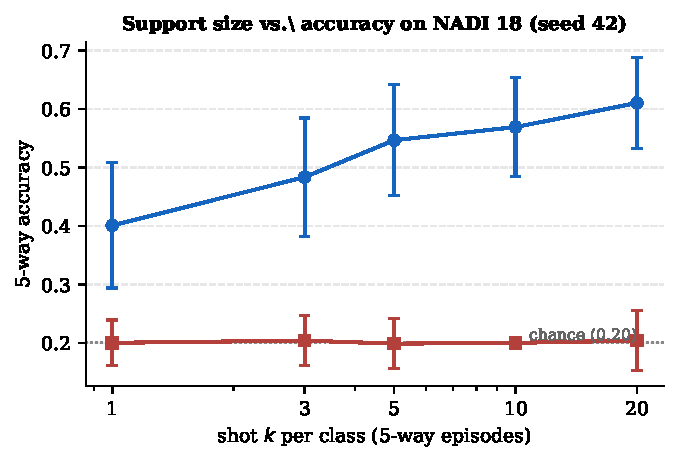
\includegraphics[width=0.95\linewidth]{figs/figA_shotcurve.pdf}
\caption{\textbf{Support-size sweep on NADI 18 (5-way, seed 42)}
(Figure~A.1). FineTune stays at chance ($0.199$--$0.204$) for
every $k$, while ProtoNet improves monotonically
($0.401{\rightarrow}0.611$); the curves never cross.}
\label{fig:A1-shotcurve}
\end{figure}

\begin{table}[t]
\centering\scriptsize
\begin{tabular}{lccccc}
\toprule
$k$ & 1 & 3 & 5 & 10 & 20 \\
\midrule
FineTune  & 0.200 & 0.204 & 0.199 & 0.200 & 0.204 \\
ProtoNet  & 0.401 & 0.484 & 0.547 & 0.569 & 0.611 \\
\bottomrule
\end{tabular}
\caption{\textbf{Support-size sweep on NADI 18 (5-way, seed 42).}
FineTune stays at chance throughout; ProtoNet improves monotonically.}
\label{tab:A1-shotcurve}
\end{table}

\subsection{Table~A.7: MARBERT encoder sanity check}
Same protocol on amgadhasan 5-city (where MARBERT's tweet-domain
pre-training should help), using the local marbertv2 weights
(hidden $768$, last $4$ encoder layers unfrozen).
$5$-way $\times\{1,5\}$-shot with seed 42.

\begin{table}[t]
\centering\scriptsize
\begin{tabular}{lcccccc}
\toprule
& \multicolumn{3}{c}{MARBERT (amgadhasan)} & \multicolumn{3}{c}{AraBERT ref.} \\
\cmidrule(lr){2-4} \cmidrule(lr){5-7}
Method & 1-shot & 5-shot & $\Delta$(5--1) & 1-shot & 5-shot & $\Delta$(5--1) \\
\midrule
FineTune  & 0.204 & 0.204 & $0.000$ & 0.202 & 0.192 & $-0.010$ \\
ProtoNet  & 0.778 & 0.863 & $+0.085$ & 0.593 & 0.768 & $+0.175$ \\
SCP-LPA   & 0.809 & 0.872 & $+0.063$ & 0.641 & 0.785 & $+0.144$ \\
\bottomrule
\end{tabular}
\caption{\textbf{MARBERT replicates the collapse pattern.}
FineTune stays at chance; metric-learning gains persist or strengthen.}
\label{tab:A7-marbert}
\end{table}

\subsection{Table~A.8: Reverse transfer (amgadhasan $\to$ NADI 5)}
Train on amgadhasan 5-city (source) and evaluate on NADI 5-way
(target) with the source \emph{prior} carried over (same
$5{\times}5$ shape, mismatched city-vs-group semantics). Seed 42.

\begin{table}[t]
\centering\scriptsize
\begin{tabular}{lccc}
\toprule
Method & 1-shot & 5-shot & note \\
\midrule
ProtoNet                       & 0.374 & 0.518 & (no prior) \\
SCP                            & 0.369 & 0.492 & SupCon weight $1.0$ \\
SCP-LPA (\emph{source} prior) & 0.372 & 0.492 & $\Delta{=}0.0002$ vs.\ SCP \\
\bottomrule
\end{tabular}
\caption{\textbf{Reverse transfer: source prior is corpus-specific.}
Carrying the source city prior onto coarse-group episodes changes
SCP-LPA's result by $\le 0.003$ (effectively zero); the
$\Delta$(5--1) gaps also stay small. SCP's SupCon objective
itself does not help in the reverse direction either---the
small amgad corpus gives SupCon little structure to transfer.}
\label{tab:A8-reverse}
\end{table}

\section{Limitations and Future Work}
\paragraph{LLM baselines.} We were unable to run real GPT-4o or Jais-30B
without API access. Our TF-IDF proxy ($0.27$ on NADI 18 1-shot)
shows that simple lexical baselines are far worse than neural
methods, suggesting that LLM 1-shot performance may be unreliable.
A full LLM comparison is left for future work.

\paragraph{Language generalization.} The current benchmark focuses on
Arabic. The framework generalises to other long-tail dialect
identification settings (Hindi, Mandarin, Spanish) but these are
not evaluated.

\end{document}